\documentclass[11pt, a4paper]{report}
\usepackage[left=3cm,top=3cm,bottom=3cm,right=3cm]{geometry}
\usepackage{amsmath}
\usepackage{amssymb}
\usepackage{amsfonts}
\usepackage{graphicx}
\usepackage{tikz}
\usepackage{pgfplots}
\usepackage{xcolor}
\usepackage{float}
\usepackage{fancyhdr}
\usepackage{setspace}
\usepackage{listings}
\usepackage{courier}
\usepackage{algorithm}
\usepackage{algorithmic}
\usepackage{microtype}
\usepackage{enumitem}

\lstset{
    basicstyle=\footnotesize\ttfamily,
    breaklines=true
}

\usepackage{titlesec}

\titlespacing*{\chapter}{0pt}{0pt}{1em}

\titleformat{\chapter}
  {\normalfont\Huge\bfseries}
  {\thechapter.}{1em}{}

 \usepackage[colorlinks=true,
            linkcolor=blue,
            urlcolor=blue,
            citecolor=blue]{hyperref}

 
\title{Design and Architecture Specification for the Wi-Fi Steering Engine}
\author{\textit{Team 15}: System Architecture Team}
\date{November 2025}

\begin{document}
\maketitle
\newpage
\tableofcontents
\newpage

\chapter{Introduction}

This document defines the design and architecture of the Wi-Fi Steering Engine. It serves as a formal technical reference for how the system collects link and beacon measurements, computes real-time Quality-of-Experience (QoE) scores, ranks neighboring access points, and triggers automated roaming decisions using IEEE 802.11v BSS Transition Management (BSS-TM).

\section{System Purpose}

The Wi-Fi Steering Engine addresses the problem of suboptimal client connectivity in dense wireless deployments. Clients often remain associated with access points that provide degraded service due to distance, interference, or load, even when better alternatives exist nearby. The engine solves this by continuously monitoring station conditions and proactively steering devices to better-performing access points.

The system operates as a closed-loop control system: measurements feed into analytics, analytics inform decisions, and decisions trigger actions through the AP controller. All components operate independently but coordinate through shared data stores.

\section{Architectural Components}

The architecture combines several independent subsystems connected through shared in-memory databases and scheduled processing loops:

\begin{itemize}
    \item \textbf{Measurement Generation}: Link Measurement, Beacon Measurement, and station fetch operations driven by periodic schedulers.
    \item \textbf{Metrics Layer}: Computes QoE and Neighbor Ranking from incoming measurements.
    \item \textbf{Transition Management Engine}: Determines when and where to steer stations based on QoE thresholds and ranked neighbor lists.
    \item \textbf{Controller Interface}: Issues 802.11v commands to the AP.
    \item \textbf{StateAPI}: An HTTP server exporting station metrics with anonymized identifiers.
    \item \textbf{Dashboards}: Real-time monitoring of all subsystems, multiplexed through SocketPool.
    \item \textbf{Storage Layer}: In-memory DBs with periodic snapshotting.
\end{itemize}

Each subsystem operates independently but exchanges data via the databases and message interfaces. All schedulers run as isolated threads with strict intervals to ensure predictable timing and avoid race conditions.

\section{Design Goals}

The primary design goal is to maintain stable, high-quality client connectivity by continuously evaluating per-station conditions and steering devices toward better-performing access points when needed. The system must operate with minimal latency, handle hundreds of concurrent stations, and expose detailed state information for monitoring and debugging.

One capability remains partially implemented: post-roam QoE delta analysis. The system does not yet factor the improvement...or degradation...after a steering event back into its decision logic. This limits adaptive learning but is planned for a future release.

\chapter{System Architecture Overview}

\section{Component Organization}

The system is organized into functional layers that process data in a pipeline fashion. Raw measurements enter at the bottom layer, flow through analytics processing, and emerge as steering decisions at the top layer. This unidirectional flow simplifies reasoning about system behavior and enables independent testing of each layer.

\subsection{Measurement Layer}

This layer handles all data acquisition from the wireless infrastructure. It consists of three primary mechanisms:

\begin{enumerate}
    \item \textbf{Link Measurement}: Issues IEEE 802.11k Link Measurement requests to stations and processes the resulting reports. These reports contain transmit power, link margin, and RSSI data that characterize the current connection quality.
    
    \item \textbf{Beacon Measurement}: Requests 802.11k Beacon Reports from clients, which contain per-neighbor RSSI values, channel utilization, and station counts. This data enables the system to understand what alternative APs are visible to each client.
    
    \item \textbf{Station Statistics}: Polls the AP controller for per-station counters including TX/RX byte counts, retry rates, FCS error rates, inactive time, and current bitrates. These statistics provide insight into throughput, reliability, and activity levels.
\end{enumerate}

All measurement operations are triggered by periodic schedulers rather than events. This ensures consistent timing and prevents measurement floods when many stations connect simultaneously.

\subsection{Analytics Layer}

The analytics layer transforms raw measurements into actionable metrics. It implements two primary computations:

\begin{enumerate}
    \item \textbf{QoE Computation}: Combines signal strength, throughput, reliability, latency, and activity metrics into a single normalized quality score between 0 and 1. The computation uses weighted averaging with configurable weights that reflect the relative importance of each dimension.
    
    \item \textbf{Neighbor Ranking}: Processes beacon measurement reports to produce a sorted list of candidate APs for each station. The ranking considers neighbor RSSI, estimated capacity, and channel load to identify the best steering targets.
\end{enumerate}

Both computations maintain historical data to detect trends and volatility. Moving averages smooth out short-term fluctuations, while linear regression slopes indicate whether conditions are improving or degrading over time.

\subsection{Decision Layer}

The decision layer implements the steering policy. The Transition Management Engine examines each station's current QoE score and, if it falls below the configured threshold (0.55), constructs a BSS Transition Management request containing the ranked list of candidate APs.

The engine applies several guards before steering:
\begin{itemize}
    \item Stations with QoE above threshold are not steered
    \item Stations without ranked neighbors cannot be steered
    \item Recent steering events are rate-limited to prevent oscillation
\end{itemize}

\subsection{Control Layer}

The control layer translates steering decisions into IEEE 802.11v BSS-TM frames and sends them through the AP controller. It handles the vendor-specific details of controller communication while presenting a uniform interface to the decision layer.

The \texttt{BssTmRequestBuilder} constructs properly formatted BSS-TM requests with the \texttt{PREFERRED\_CAND\_LIST\_INCLUDED} mode, which includes the ranked neighbor list. The client firmware uses this list to select its next AP.

\subsection{Management Layer}

The management layer provides observability and persistence:

\begin{itemize}
    \item \textbf{StateAPI} exposes current system state via HTTP JSON endpoints with anonymized station identifiers
    \item \textbf{Dashboards} provide real-time WebSocket feeds of measurement reports, QoE updates, and steering events
    \item \textbf{Snapshot Manager} periodically serializes all in-memory databases to disk for recovery after restart
\end{itemize}

\section{Data Flow}

Data flows through the system in a strict pipeline:

\begin{enumerate}
    \item Schedulers trigger measurement requests at fixed intervals
    \item Measurement reports arrive and are stored in the measurement database
    \item Analytics schedulers periodically read measurements and compute QoE/ranking
    \item Computed metrics are stored in dedicated databases
    \item The transition management scheduler reads metrics and makes steering decisions
    \item Steering commands are sent to the controller
    \item All state changes are visible through the StateAPI and dashboards
\end{enumerate}

This pipeline architecture ensures that each stage operates on consistent snapshots of data without worrying about concurrent modifications. Databases implement versioning to support lock-free reads while schedulers update data.

\section{Threading Model}

The system uses one thread per major scheduler to ensure timing independence:

\begin{itemize}
    \item Link Measurement Scheduler thread
    \item Beacon Measurement Scheduler thread  
    \item QoE Computation Scheduler thread
    \item Neighbor Ranking Scheduler thread
    \item BSS Transition Scheduler thread
\end{itemize}

Additional threads handle HTTP requests (StateAPI), WebSocket connections (dashboards), and controller communication. All inter-thread communication occurs through the shared databases, which use locking primitives to ensure consistency.

\chapter{Schedulers and Data Acquisition}

\section{Scheduler Framework}

All schedulers follow the same execution pattern: wake at fixed intervals, fetch relevant data, perform computation, store results, and return to sleep. This deterministic timing simplifies debugging and makes system behavior predictable.

Each scheduler maintains internal state including:
\begin{itemize}
    \item Last execution timestamp
    \item Execution count  
    \item Error counters
    \item Performance metrics (min/max/avg execution time)
\end{itemize}

\section{Link Measurement Scheduler}

The Link Measurement Scheduler maintains up-to-date connection quality data for all stations. It operates as follows:

\begin{enumerate}
    \item Fetch the list of currently connected stations from the controller
    \item For each station, check if a recent link measurement exists in the database
    \item If no recent measurement exists (or the last one is stale), construct a Link Measurement request:
    
    \begin{verbatim}
    req_link_measurement(LinkMeasurementCommandBuilder(station.mac))
    \end{verbatim}
    
    \item Send the request through the controller interface
    \item Mark the request timestamp to avoid duplicate requests
\end{enumerate}

The measurement report processing happens asynchronously. When a station responds with an 802.11k Link Measurement Report frame, the controller forwards it to the engine, which parses the frame and extracts:

\begin{itemize}
    \item RSSI (Received Signal Strength Indicator)
    \item Transmit power used by the station
    \item Link margin indicating fade margin before packet loss
    \item Receive antenna configuration
\end{itemize}

These values are stored in the Link Measurement database with a timestamp. The QoE computation scheduler later reads these values when calculating signal quality scores.

\section{Beacon Measurement Scheduler}

The Beacon Measurement Scheduler gathers information about what APs each station can see and how strong those signals are. This data is essential for building ranked neighbor lists.

The scheduler issues 802.11k Beacon Report requests using:

\begin{verbatim}
RequestBeaconCommandBuilder(station_mac)
    .set_measurement_params(operating_class, channel, duration)
\end{verbatim}

Key parameters include:
\begin{itemize}
    \item \textbf{Operating Class}: Defines the frequency band (2.4 GHz, 5 GHz, etc.)
    \item \textbf{Channel}: Specific channel to measure, or 255 for all channels
    \item \textbf{Duration}: How long to spend measuring (in 802.11 Time Units)
\end{itemize}

When a station responds, the beacon report contains measurements for multiple neighboring APs. Each neighbor entry includes:
\begin{itemize}
    \item BSSID (MAC address of the AP)
    \item RCPI (Received Channel Power Indicator) - equivalent to RSSI
    \item RSNI (Received Signal-to-Noise Indicator)
    \item Channel utilization
    \item Number of associated stations
\end{itemize}

These reports are stored in the Beacon Measurement database, aggregated across multiple measurement cycles to reduce variance from temporary conditions.

\section{QoE Scheduler}

The QoE Scheduler is responsible for periodically recomputing quality scores for all active stations. It executes at the shortest interval (typically every 5 seconds) to ensure scores reflect current conditions.

The execution sequence is:

\begin{verbatim}
QoE.update()
\end{verbatim}

This method:
\begin{enumerate}
    \item Fetches recent link measurements for all stations
    \item Fetches station statistics (throughput, retry rates, etc.)
    \item For each station with sufficient data, calls the QoE computation function
    \item Stores the computed QoE score and its component breakdown
    \item Updates the historical model (moving average, trend, volatility)
\end{enumerate}

The historical model tracks QoE evolution over time. It maintains:
\begin{itemize}
    \item A sliding window of the last N QoE samples (typically N=10)
    \item A moving average computed as: $\bar{Q} = \frac{1}{N}\sum_{i=1}^{N} Q_i$
    \item A trend value computed via linear regression: $\text{trend} = \text{slope}(Q_1, Q_2, \ldots, Q_N)$
    \item Volatility computed as sample variance: $\sigma^2 = \frac{1}{N}\sum_{i=1}^{N}(Q_i - \bar{Q})^2$
\end{itemize}

These metrics help distinguish temporary fluctuations from genuine degradation. A station with high volatility may not need steering, while one with consistently low QoE or negative trend is a strong steering candidate.

\section{Neighbor Ranking Scheduler}

The Neighbor Ranking Scheduler processes beacon measurement reports to build sorted candidate lists for steering. It executes:

\begin{verbatim}
NeighborRanking.update()
\end{verbatim}

For each station, this method:
\begin{enumerate}
    \item Retrieves all beacon reports from the last measurement window
    \item Groups measurements by neighbor BSSID
    \item Computes aggregate statistics (average RSSI, load, etc.)
    \item Applies the neighbor ranking algorithm (detailed in Chapter 5)
    \item Stores the sorted neighbor list in the ranking database
\end{enumerate}

The ranking database maps each station MAC to its current ranked neighbor list. This list is referenced by the Transition Management Engine when constructing steering requests.

\section{BSS Transition Scheduler}

The BSS Transition Scheduler implements the steering policy by invoking:

\begin{verbatim}
TransitionManagementEngine.run()
\end{verbatim}

This method iterates over all connected stations and applies the steering decision logic described in Chapter 6. It runs at the longest interval (typically 60 seconds) to avoid excessive steering and allow time for roaming to complete.

\chapter{Quality of Experience (QoE) Computation}

Quality of Experience quantifies how well the network serves the client across
two independent dimensions:

\begin{itemize}
    \item \textbf{AP-side QoE ($Q_{\text{AP}}$)}: Measures wireless link quality based on
    physical and MAC-layer metrics.
    \item \textbf{Transport-layer QoE ($Q_{\text{transport}}$)}: Measures end-to-end
    performance using TCP RTT, retransmissions, and throughput.
\end{itemize}

These two QoEs are \textbf{computed independently}. Each captures different
aspects of the client experience, and together they provide a complete view of
both RF conditions and transport-layer behavior.

\section{AP-Side QoE}

AP-side QoE, denoted $Q_{\text{AP}}$, is computed from five normalized
components:

\begin{itemize}
    \item $S$: Signal quality score
    \item $T$: Throughput score
    \item $R$: Reliability score
    \item $L$: Latency/Responsiveness score
    \item $A$: Activity score
\end{itemize}

The AP-side QoE is given by:

\begin{equation}
Q_{\text{AP}} = w_S S + w_T T + w_R R + w_L L + w_A A
\end{equation}

Weights:

\[
w_S = 0.28,\quad
w_T = 0.32,\quad
w_R = 0.15,\quad
w_L = 0.15,\quad
w_A = 0.10
\]

\subsection{Signal Quality Component}

Signal quality uses RSSI to measure RF link strength. RSSI is mapped to the
range $[0,1]$:

\begin{equation}
S = \text{clamp}\left(\frac{\text{RSSI} - (-90)}{60}, 0, 1\right)
\end{equation}

Values:
\begin{itemize}
    \item RSSI $\le -90$ dBm $\rightarrow S = 0$
    \item RSSI $\ge -30$ dBm $\rightarrow S = 1$
\end{itemize}

Example:
\[
\text{RSSI} = -50 \Rightarrow S = 0.67
\]

\subsection{Throughput Component}

Throughput is estimated using the geometric mean of uplink and downlink
bitrates:

\begin{equation}
T = \text{clamp}\left(
\frac{\sqrt{\text{tx\_bitrate} \cdot \text{rx\_bitrate}}}{\text{phy\_peak}},
0, 1 \right)
\end{equation}

Example:
\[
T = \frac{300}{866} = 0.35
\]

\subsection{Reliability Component}

Reliability captures link stability using retry and FCS error rates:

\begin{equation}
R = 1 - (\alpha \cdot \text{retry\_rate} + \beta \cdot \text{fcs\_rate})
\end{equation}

\[
\alpha = 0.6,\qquad \beta = 0.4
\]

Example:
\[
R = 1 - (0.006 + 0.002) = 0.992
\]

\subsection{Latency Component}

Latency is estimated via the inactivity timer:

\begin{equation}
L = \text{clamp}\left(
1 - \frac{\text{inactive\_msec}}{5000},\,0,\,1
\right)
\end{equation}

Example:
\[
\text{inactive}=2500\text{ ms} \Rightarrow L = 0.50
\]

\subsection{Activity Component}

Activity captures station usage intensity:

\begin{equation}
A = \text{clamp}\left(
\frac{\text{tx\_packets} + \text{rx\_packets}}{\text{max\_frames}},
0,1
\right)
\end{equation}

Stations above \texttt{max\_frames} saturate at $A=1$.

\section{TCP QoE (Updated)}


\begin{enumerate}
    \item TCP packet capture using \texttt{tcpdump}
    \item Raw metric extraction from TCP fields
    \item Normalization with parameterized constants
    \item Final QoE computation
\end{enumerate}



\subsection{Part 1: TCP Packet Capture}


\begin{lstlisting}[language=bash]
# Start capture
sudo tcpdump -i br0 -s 0 -w wifi_tcp.pcap 'tcp' &

# Generate traffic on client

# Stop: Ctrl+C
\end{lstlisting}


\subsection{Part 2: TCP Layer Fields}

\subsubsection{Core TCP Variables}

For each packet $p_i$, extract:

\begin{description}[leftmargin=2.2cm, style=nextline]

  \item[$t_i$] Timestamp (sec) —\texttt{pkt.time}

  \item[$\text{sport}_i$] Source Port — \texttt{pkt[TCP].sport}

  \item[$\text{dport}_i$] Destination Port — \texttt{pkt[TCP].dport}

  \item[$\text{seq}_i$] Sequence Number — \texttt{pkt[TCP].seq}

  \item[$\text{ack}_i$] Acknowledgment Number — \texttt{pkt[TCP].ack}

  \item[$\text{len}_i$] Payload Length (bytes) — \texttt{len(bytes(pkt[TCP].payload))}

  \item[$\text{TSval}_i$] Timestamp Value (ticks) — \texttt{pkt[TCP].options}

  \item[$\text{TSecr}_i$] Timestamp Echo (ticks) — \texttt{pkt[TCP].options}

\end{description}


\subsubsection{Flow Identification}

TCP flow identified by 2-tuple:

\begin{equation}
\text{Flow} = (\text{sport}, \text{dport})
\end{equation}

\subsection{Part 3: Raw Metric Extraction}

\subsubsection{Metric 1: Round-Trip Time (RTT)}

\textbf{RTT from TCP Timestamp Option (RFC 1323)}

\begin{equation}
\text{RTT}_{i,j}^{\text{TS}} = t_j - \text{TSval}_{i}
\end{equation}

Where:
\begin{itemize}
    \item $t_j$ = arrival time of ACK packet (seconds)
    \item $\text{TSval}_{i}$ = timestamp value from data packet
\end{itemize}

\subsubsection{Metric : RTT Jitter (Variability)}

\textbf{Formula}

Jitter is the standard deviation of RTT samples:

\begin{equation}
\text{Jitter} = \sigma_{\text{RTT}} = \sqrt{\frac{1}{M-1} \sum_{k=1}^{M} (\text{RTT}_k - \overline{\text{RTT}})^2}
\end{equation}

Where:
\begin{itemize}
    \item $M$ = number of RTT samples
    \item $\overline{\text{RTT}}$ = mean RTT
\end{itemize}


\subsubsection{Metric 3: Packet Loss Rate}

\textbf{Retransmission Detection}

A packet is retransmitted if same TCP sequence number appears twice on same flow:

\begin{equation}
\text{seq}_i \in \text{SEEN}[\text{flow}_i] \Rightarrow \text{retransmission}
\end{equation}

\textbf{Loss Rate Formulas}

Per-flow loss rate:

\begin{equation}
\text{Loss}[\text{flow}] = \frac{\text{RETRANS}[\text{flow}]}{\text{TOTAL}[\text{flow}]} \times 100\%
\end{equation}

Overall loss rate:

\begin{equation}
\text{Loss}_{\text{total}} = \frac{\sum_f \text{RETRANS}[f]}{\sum_f \text{TOTAL}[f]} \times 100\%
\end{equation}



\subsubsection{Metric 4: Throughput}

\textbf{Formula}

Throughput from total TCP payload:

\begin{equation}
B_{\text{total}} = \sum_{p_i: \text{len}_i > 0} \text{len}_i
\end{equation}

Capture duration:

\begin{equation}
T_{\text{capture}} = t_{\max} - t_{\min}
\end{equation}

Throughput in Mbps:

\begin{equation}
\text{Throughput}_{\text{Mbps}} = \frac{B_{\text{total}} \times 8}{T_{\text{capture}} \times 10^6}
\end{equation}



\subsection{Part 4: Normalization with Parameters}

\subsubsection{RTT Normalization}

\textbf{Formula with Parameter}

\begin{equation}
\boxed{Q_{\text{lat}}(\text{RTT}) = \frac{1}{1 + \frac{\text{RTT}}{R_0}}}
\end{equation}

Where $R_0$ is the RTT reference parameter (default: 50 ms).

\textbf{Why This Form}

\begin{itemize}
    \item Continuous degradation (no threshold)
    \item Logarithmic perception (Weber's law)
    \item Simple computation
    \item Tunable via $R_0$
\end{itemize}

\subsubsection{Jitter Normalization}

\textbf{Formula with Parameter}

\begin{equation}
\boxed{Q_{\text{jitter}}(\text{Jitter}) = \frac{1}{1 + \frac{\text{Jitter}}{J_0}}}
\end{equation}

Where $J_0$ is the jitter reference parameter

\subsubsection{Loss Rate Normalization}

\textbf{Formula with Parameter}

\begin{equation}
\boxed{Q_{\text{loss}}(\text{Loss}) = \frac{1}{1 + L_0 \times \text{Loss}}}
\end{equation}

Where:
\begin{itemize}
    \item $L_0$ = loss steepness parameter
    \item $\text{Loss}$ = loss rate in decimal 
\end{itemize}




\subsubsection{Throughput Normalization}

\textbf{Formula with Parameter}

\begin{equation}
\boxed{Q_{\text{tput}}(\text{Throughput}) = \frac{\text{Throughput}}{T_0 + \text{Throughput}}}
\end{equation}

Where $T_0$ is the throughput reference parameter

\textbf{Why Diminishing Returns}

Each additional Mbps has less impact. Logarithmic form captures real utility.

\subsection{Part 5: Final QoE Computation}

\subsubsection{QoE Formula}

\begin{equation}
\boxed{Q_{\text{QoE}} = w_{\text{lat}} \cdot Q_{\text{lat}} + w_{\text{jitter}} \cdot Q_{\text{jitter}} + w_{\text{loss}} \cdot Q_{\text{loss}} + w_{\text{tput}} \cdot Q_{\text{tput}}}
\end{equation}



\subsection{Summary of Formulas with Parameters}

\subsubsection{Raw Metrics (TCP Only)}

\begin{equation}
\boxed{\text{RTT} = t_{\text{ack}} - \text{TSval}_{\text{data}}}
\end{equation}

\begin{equation}
\boxed{\text{Jitter} = \sqrt{\frac{1}{M-1} \sum_{k=1}^{M} (\text{RTT}_k - \overline{\text{RTT}})^2}}
\end{equation}

\begin{equation}
\boxed{\text{Loss} = \frac{\text{duplicate sequences}}{\text{total packets}} \times 100\%}
\end{equation}

\begin{equation}
\boxed{\text{Throughput} = \frac{\sum \text{payload bytes} \times 8}{T_{\text{capture}} \times 10^6} \text{ Mbps}}
\end{equation}

\subsubsection{Normalization with Parameters}

\begin{equation}
\boxed{Q_{\text{lat}} = \frac{1}{1 + \text{RTT}/R_0}}
\end{equation}

\begin{equation}
\boxed{Q_{\text{jitter}} = \frac{1}{1 + \text{Jitter}/J_0}}
\end{equation}

\begin{equation}
\boxed{Q_{\text{loss}} = \frac{1}{1 + L_0 \times \text{Loss}}}
\end{equation}

\begin{equation}
\boxed{Q_{\text{tput}} = \frac{\text{Throughput}}{T_0 + \text{Throughput}}}
\end{equation}

\subsubsection{Final QoE with Weights}

\begin{equation}
\boxed{Q_{\text{QoE}} = w_{\text{lat}} Q_{\text{lat}} + w_{\text{jitter}} Q_{\text{jitter}} + w_{\text{loss}} Q_{\text{loss}} + w_{\text{tput}} Q_{\text{tput}}}
\end{equation}

Default weights: $(0.25, 0.25, 0.35, 0.15)$


\section{Historical Trend Analysis}

While instantaneous QoE values provide a snapshot of performance, wireless
conditions often fluctuate due to mobility, interference, and variations in
traffic load. To better understand long-term behavior, the system maintains a
history of QoE samples for each station. This enables the controller to
distinguish between temporary fluctuations and persistent degradation.

Three metrics are tracked: moving average, trend, and volatility.

\subsection{Moving Average}

The moving average smooths short-term noise and provides a stable baseline for
QoE evaluation. It is computed over the last $k$ samples:

\begin{equation}
\bar{Q}_t = \frac{1}{k} \sum_{i=0}^{k-1} Q_{t-i}
\end{equation}

A larger $k$ makes the average more stable but slower to react to changes. A
typical value is $k=10$ samples.

\subsection{Trend Computation}

The trend metric represents the direction and rate of QoE change over time. It
is computed using the slope of a least-squares linear regression over the last
$k$ samples:

\begin{equation}
\text{trend} =
\frac{
k \sum_{i=1}^{k} i Q_i -
(\sum_{i=1}^{k} i)(\sum_{i=1}^{k} Q_i)
}{
k \sum_{i=1}^{k} i^2 -
(\sum_{i=1}^{k} i)^2
}
\end{equation}

A positive trend indicates improving conditions (e.g., station moving closer to
AP, reduced interference), while a negative trend signals progressive
deterioration. This metric is particularly useful for early detection of
coverage holes or congestion buildup.

\subsection{Volatility}

Volatility measures the short-term stability of QoE. High volatility indicates
rapid fluctuations caused by interference, bursty traffic, hidden-node
collisions, or client mobility.

It is computed as the variance of recent QoE values:

\begin{equation}
\sigma^2 =
\frac{1}{k}
\sum_{i=0}^{k-1}
(Q_{t-i} - \bar{Q}_t)^2
\end{equation}

Low volatility combined with poor QoE suggests persistent problems (e.g.,
weak signal, overloaded AP), while high volatility suggests transient issues
that may resolve without client steering.

\section{Post-Roam QoE Delta Analysis}

To evaluate the effectiveness of a steering decision, the system compares QoE
before and after a client roams from AP$_1$ to AP$_2$. This allows the
controller to validate whether the steering action improved or degraded the
user's experience.

The QoE delta is computed as:

\begin{equation}
\Delta Q = Q(\text{AP}_2) - Q(\text{AP}_1)
\end{equation}

A positive $\Delta Q$ indicates that the new AP provides better service,
justifying the roam. A negative $\Delta Q$ suggests that the client was moved to
a worse AP, which can trigger corrective actions or adjustments to the steering
policy.

Because QoE is computed independently for both AP-side performance
($Q_{\text{AP}}$) and transport-layer performance ($Q_{\text{transport}}$), the
controller may evaluate:

\[
\Delta Q_{\text{AP}} \quad \text{and} \quad \Delta Q_{\text{transport}}
\]

This separation helps identify whether improvements are due to RF conditions
(e.g., better SNR, lower retries) or due to transport-layer characteristics
(e.g., lower RTT, reduced congestion).



\chapter{Neighbor Ranking Algorithm}

\section{Ranking Overview}

Neighbor ranking determines which APs are suitable steering targets for each station. The algorithm processes beacon measurement reports to score and sort candidate APs based on predicted performance.

The ranking must balance competing factors:
\begin{itemize}
    \item Strong signal (high RSSI) indicates good RF conditions
    \item High capacity means the AP can handle additional load
    \item Low current load suggests available airtime
\end{itemize}

\section{Scoring Formula}

For each neighbor AP visible to a station, the score is computed as:

\begin{equation}
N_i = \gamma_1 \cdot \text{RSSI}_i + \gamma_2 \cdot \text{capacity}_i - \gamma_3 \cdot \text{load}_i
\end{equation}

With weights:
\begin{equation}
\gamma_1 = 0.55,\quad \gamma_2=0.35,\quad \gamma_3=0.10
\end{equation}

All components are normalized to comparable ranges before weighting.

\subsection{RSSI Component}

RSSI from beacon reports is converted to a 0-1 score using the same mapping as the QoE signal component:

\begin{equation}
\text{RSSI}_{\text{score}} = \text{clamp}\left(\frac{\text{RCPI}/2 - 110 - (-90)}{60}, 0, 1\right)
\end{equation}

Where RCPI (Received Channel Power Indicator) from the beacon report is converted to dBm by dividing by 2 and subtracting 110.

RSSI receives the highest weight (0.55) because RF quality is the primary constraint on achievable throughput. An AP with poor RSSI will not perform well regardless of its capacity or load.

\subsection{Capacity Component}

Capacity estimates the maximum throughput the AP can provide based on:
\begin{itemize}
    \item Channel width (20/40/80/160 MHz)
    \item PHY type (802.11n/ac/ax)
    \item Spatial streams supported
\end{itemize}

This information comes from the AP's beacon frame capabilities. The capacity score is normalized relative to the best technology available in the deployment.

Capacity weight is 0.35, reflecting that a high-capacity AP (e.g., 802.11ax with 80 MHz) can support higher throughput than an older AP even at similar RSSI.

\subsection{Load Component}

Channel load comes from the channel utilization field in beacon reports. It represents the fraction of time the channel is busy:

\begin{equation}
\text{load}_{\text{score}} = \frac{\text{channel\_utilization}}{255}
\end{equation}

The score is subtracted (note the negative weight $\gamma_3 = 0.10$) because high load is undesirable. An AP at 90\% utilization will provide worse performance than one at 20\% utilization.

Load receives the lowest weight because momentary utilization fluctuates significantly. Signal and capacity are more stable predictors.

\section{Neighbor Aggregation}

Beacon reports may arrive from multiple measurement cycles. The system aggregates measurements for each neighbor BSSID:

\begin{itemize}
    \item Average RSSI across all reports
    \item Most recent capacity information
    \item Average channel load
\end{itemize}

This aggregation reduces the impact of single anomalous measurements. A neighbor that consistently appears with strong RSSI across multiple reports is more reliable than one with a single strong measurement.

\section{Sorting and Selection}

After scoring all neighbors, they are sorted in descending order of score $N_i$. The top-ranked neighbors become the candidate list for BSS-TM requests.

The system may apply additional filters:
\begin{itemize}
    \item Minimum RSSI threshold (e.g., reject neighbors below -80 dBm regardless of score)
    \item Band preference (e.g., prefer 5 GHz over 2.4 GHz when scores are close)
    \item Same-SSID requirement (only steer within the same network)
\end{itemize}

The final ranked list is stored in the Neighbor Ranking database, indexed by station MAC address. This list is referenced by the Transition Management Engine when constructing steering requests.

\section{Future Enhancement: Historical Performance}

Currently, ranking is purely based on predicted performance from measurements. The planned enhancement would incorporate actual historical performance:

\begin{equation}
N_i = \gamma_1 \cdot \text{RSSI}_i + \gamma_2 \cdot \text{capacity}_i - \gamma_3 \cdot \text{load}_i + \gamma_4 \cdot \text{history}_i
\end{equation}

Where \texttt{history}$_i$ represents the average post-roam $\Delta Q$ when this station (or similar stations) previously roamed to AP$_i$. This would enable adaptive learning from steering outcomes.

\chapter{Transition Management Logic}

\section{Steering Decision Process}

The Transition Management Engine implements the steering policy by examining each station and deciding whether to issue a BSS-TM request. The decision logic balances the need to improve poor connections against the disruption of unnecessary roaming.

\subsection{Decision Algorithm}

For each connected station, the engine executes:

\begin{algorithmic}[1]
\STATE station $\gets$ next connected station
\STATE qoe $\gets$ fetch current QoE(station)
\IF{qoe is None}
    \STATE skip \COMMENT{No QoE data yet}
\ENDIF
\IF{qoe.score $>$ 0.55}
    \STATE skip \COMMENT{QoE acceptable}
\ENDIF
\STATE neighbors $\gets$ fetch ranked neighbors(station)
\IF{neighbors is empty}
    \STATE skip \COMMENT{No steering candidates}
\ENDIF
\STATE request $\gets$ build\_bss\_tm\_request(station, neighbors)
\STATE controller.send(request)
\STATE log\_steering\_event(station, qoe, neighbors)
\end{algorithmic}

\section{QoE Threshold}

The threshold value of 0.55 represents the point below which user experience is considered degraded. This value was chosen to trigger steering before conditions become severe enough to cause application failures or disconnections.

The threshold is intentionally conservative (neither too high nor too low):
\begin{itemize}
    \item Too high (e.g., 0.8): Causes excessive steering of marginally suboptimal connections
    \item Too low (e.g., 0.3): Waits until connections are severely degraded before steering
\end{itemize}

At QoE = 0.55, a typical station might have:
\begin{itemize}
    \item RSSI around -65 to -70 dBm (marginal signal)
    \item Throughput at 40-50\% of peak
    \item Some retries but not excessive
    \item Generally usable but noticeably suboptimal performance
\end{itemize}

\section{BSS Transition Request Construction}

When the engine decides to steer a station, it constructs an IEEE 802.11v BSS Transition Management request using:

\begin{verbatim}
BssTmRequestBuilder(
    sta_addr=mac,
    req_mode=PREFERRED_CAND_LIST_INCLUDED,
    neighbors=nbs
)
\end{verbatim}

The request contains several key fields:

\subsection{Request Mode}

The \texttt{PREFERRED\_CAND\_LIST\_INCLUDED} mode tells the client that the frame includes a list of recommended APs. The client firmware considers this list when selecting its next association target. Other possible modes include:

\begin{itemize}
    \item \texttt{ABRIDGED}: No candidate list, client chooses independently
    \item \texttt{DISASSOC\_IMMINENT}: Warn client of impending disconnection
    \item \texttt{BSS\_TERMINATION}: AP is shutting down
\end{itemize}

The preferred candidate list mode is used because it provides guidance without forcing a specific AP, allowing the client to factor in its own measurements and preferences.

\subsection{Neighbor List}

The neighbor list contains entries for each candidate AP, ordered by ranking score. Each entry includes:

\begin{itemize}
    \item \textbf{BSSID}: MAC address of the target AP
    \item \textbf{BSSID Info}: Capabilities flags (HT, VHT, etc.)
    \item \textbf{Operating Class}: Regulatory domain frequency band
    \item \textbf{Channel Number}: Primary channel
    \item \textbf{PHY Type}: 802.11n/ac/ax indicator
\end{itemize}

This information comes from the beacon reports and neighbor database. The client uses it to quickly find and associate with the recommended APs without performing a full scan.

\subsection{Additional Parameters}

The request may include optional parameters:

\begin{itemize}
    \item \textbf{Disassociation Timer}: If set, indicates when the AP will disconnect if the client doesn't roam (not typically used in QoE-based steering)
    \item \textbf{Validity Interval}: How long the neighbor list remains valid
    \item \textbf{BSS Termination Duration}: Used when AP is shutting down (not applicable here)
\end{itemize}

For QoE-based steering, only the neighbor list is required. The station is free to remain associated if it prefers, but is encouraged to consider the alternatives.

\section{Rate Limiting and Hysteresis}

To prevent steering oscillation, the engine implements several guards:

\subsection{Minimum Time Between Steers}

Each station has a timestamp of its last steering event. The engine will not issue a new BSS-TM request until sufficient time has elapsed (typically 120-300 seconds). This prevents rapid back-and-forth steering between APs.

\subsection{QoE Hysteresis}
The current system doesn't account for QoE Hysteresis, more experimentations are required to give any potential solution.

\subsection{Minimum RSSI Delta}

The top-ranked neighbor must have significantly better RSSI than the current AP (typically 5-10 dB improvement) to justify steering. Steering to a marginally better AP may not be worth the temporary disruption.

\section{Steering Event Logging}

Every steering decision is logged with:

\begin{itemize}
    \item Station MAC address
    \item Current AP BSSID
    \item Current QoE score and component breakdown
    \item Ranked neighbor list sent in the BSS-TM request
    \item Timestamp
\end{itemize}

These logs enable post-mortem analysis of steering behavior and provide the data needed for future post-roam QoE delta analysis.

\section{Client Response Handling}

After sending a BSS-TM request, the system monitors for the client's response. The client may:

\begin{enumerate}
    \item \textbf{Accept}: Send a BSS-TM response frame indicating it will roam, then reassociate to a neighbor
    \item \textbf{Reject}: Send a BSS-TM response frame declining to roam
    \item \textbf{Ignore}: Never respond (non-compliant or legacy client)
\end{enumerate}

The response status is logged but does not immediately affect future steering decisions. In the planned post-roam analysis feature, rejected or ignored steering requests would factor into AP ranking adjustments.

\chapter{StateAPI: HTTP Interface}

\section{API Purpose and Design}

The StateAPI subsystem exposes a read-only view of system state via HTTP endpoints. It serves several purposes:

\begin{itemize}
    \item External monitoring systems can poll for metrics
    \item Dashboards can fetch current state on demand
    \item Debugging tools can inspect station conditions
    \item Historical analysis tools can collect time-series data
\end{itemize}

The API is intentionally read-only. All configuration and control operations occur through other interfaces to maintain separation of concerns.

\section{Data Refresh Process}

Before serving any API response, the StateAPI calls:

\begin{verbatim}
self.qoe.update()
\end{verbatim}

This ensures the returned data reflects current conditions rather than stale cached values. The update recomputes QoE scores based on the most recent measurements, so API responses always represent the latest system understanding.

This synchronous update adds minimal latency (typically under 10ms for 100 stations) because the QoE computation is fast and operates on pre-fetched data from the databases.

\section{Response Structure}

Each API response follows a standard envelope format:

\begin{verbatim}
{
  "timestamp": <unix epoch seconds>,
  "status": "ok" | "error",
  "component": "StateAPI",
  "version": "1.0",
  "length": <number of station records>,
  "data": [ <station records> ]
}
\end{verbatim}

The \texttt{timestamp} field indicates when the response was generated. The \texttt{length} field allows clients to quickly determine how many station records are present without parsing the entire array.

\section{Station Record Format}

Each station in the \texttt{data} array contains:

\subsection{Identity}
\begin{verbatim}
"public_id": "A4:5E:60-9f13ab"
\end{verbatim}

The anonymized identifier (see Section 7.5 for details).

\subsection{Connection Status}
\begin{verbatim}
"connected": true | false
\end{verbatim}

Whether the station is currently associated to an AP under management.

\subsection{Signal Metrics}
\begin{verbatim}
"signal": {
  "avg_signal": -31,          // dBm
  "score": 1.0                // normalized 0-1
}
\end{verbatim}

Current RSSI and the computed signal component score.

\subsection{Throughput Metrics}
\begin{verbatim}
"throughput": {
  "tx_bitrate": 54,           // Mbps
  "rx_bitrate": 54,           // Mbps
  "score": 0.22               // normalized 0-1
}
\end{verbatim}

Current TX/RX bitrates and throughput component score.

\subsection{Reliability Metrics}
\begin{verbatim}
"reliability": {
  "tx_retry_rate": 5.9e-7,    // ratio
  "tx_failed_rate": 0.0,      // ratio
  "rx_fcs_error_rate": 0.0,   // ratio
  "score": 1.0                // normalized 0-1
}
\end{verbatim}

Retry and error rates with the computed reliability score.

\subsection{Latency Metrics}
\begin{verbatim}
"latency": {
  "inactive_msec": 2064,      // milliseconds
  "score": 1.0                // normalized 0-1
}
\end{verbatim}

Time since last frame exchange and latency component score.

\subsection{Activity Metrics}
\begin{verbatim}
"activity": {
  "total_tx_rx_packets": 79617,
  "score": 1.0                // normalized 0-1
}
\end{verbatim}

Total frame count and activity component score.

\subsection{QoE Summary}
\begin{verbatim}
"qoe": {
  "overall": 0.883,           // composite score
  "trend": "insufficient_data" | "improving" | "stable" | "degrading",
  "volatility": 0.02          // variance (if available)
}
\end{verbatim}

The final composite QoE score, trend classification, and volatility measure.

\subsection{Timestamp}
\begin{verbatim}
"timestamp": "2025-11-15T16:47:49.937132"
\end{verbatim}

ISO 8601 formatted timestamp for this station's measurement snapshot.

\section{Identifier Anonymization}

Raw MAC addresses contain device-identifying information and may be considered personally identifiable. To enable public API exposure without privacy concerns, the StateAPI anonymizes all station identifiers.

\subsection{Anonymization Algorithm}

The anonymization preserves the OUI (Organizationally Unique Identifier) portion while hashing the device-specific portion:

\begin{equation}
\text{public\_id} = \text{OUI}(\text{MAC}) \; || \; \text{``-''} \; || \; \text{H}(\text{suffix})
\end{equation}

Where:
\begin{itemize}
    \item $\text{OUI}(\text{MAC})$ extracts the first 3 bytes (6 hex digits)
    \item $\text{suffix}$ is the last 3 bytes of the MAC address
    \item $\text{H}$ is SHA-256 hash, truncated to 24 bits (6 hex digits)
\end{itemize}

For example, given MAC address \texttt{A4:5E:60:3C:F1:82}:

\begin{enumerate}
    \item OUI = \texttt{A4:5E:60} (vendor identifier, retained)
    \item Suffix = \texttt{3C:F1:82} (device-specific)
    \item Hash = \texttt{SHA256("3C:F1:82")} = \texttt{9f13ab...} (truncated)
    \item Result = \texttt{A4:5E:60-9f13ab}
\end{enumerate}

\subsection{Privacy Properties}

This scheme provides several privacy properties:

\begin{itemize}
    \item \textbf{Non-reversible}: The hash function is one-way; the original MAC cannot be recovered from the public ID
    \item \textbf{Vendor-preserving}: The OUI remains visible, allowing analysis by device manufacturer
    \item \textbf{Consistent}: The same MAC always produces the same public ID (useful for tracking across API calls)
    \item \textbf{Unlinkable}: Without knowledge of the MAC, an observer cannot link public IDs across different deployments
\end{itemize}

\subsection{Implementation}

The anonymization is performed in the \texttt{build\_station\_api\_dict()} method:

\begin{verbatim}
def anonymize_mac(mac: str) -> str:
    oui = mac[:8]  # "A4:5E:60"
    suffix = mac[9:]  # "3C:F1:82"
    hash_input = suffix.encode('utf-8')
    hash_output = hashlib.sha256(hash_input).hexdigest()
    return f"{oui}-{hash_output[:6]}"
\end{verbatim}

This function is called once per station when building the API response. The internal databases, schedulers, and decision logic continue to use the raw MAC address for all operations. Only the final API serialization step performs anonymization.

\subsection{OUI Retention Rationale}

Retaining the OUI (vendor identifier) enables useful analysis:

\begin{itemize}
    \item Identifying problematic device types (e.g., "all Apple devices have low QoE")
    \item Vendor-specific tuning (e.g., "Samsung phones respond well to 5 GHz steering")
    \item Hardware capability inference (OUI correlates with PHY capabilities)
\end{itemize}

The OUI alone does not uniquely identify a device, as millions of devices share the same vendor identifier. The privacy risk is minimal compared to the analytical value.

\section{Example API Output}

A complete API response for two stations:

\begin{verbatim}
{
  "timestamp": 1763205469.937012,
  "status": "ok",
  "component": "StateAPI",
  "version": "1.0",
  "length": 2,
  "data": [
    {
      "public_id": "0E:ED:C0-3A91E2",
      "connected": true,
      "signal": { 
        "avg_signal": -31, 
        "score": 1.0 
      },
      "throughput": { 
        "tx_bitrate": 54, 
        "rx_bitrate": 54,
        "score": 0.22 
      },
      "reliability": { 
        "tx_retry_rate": 5.9e-7,
        "tx_failed_rate": 0.0,
        "rx_fcs_error_rate": 0.0,
        "score": 1.0 
      },
      "latency": { 
        "inactive_msec": 2064, 
        "score": 1.0 
      },
      "activity": { 
        "total_tx_rx_packets": 79617, 
        "score": 1.0 
      },
      "qoe": { 
        "overall": 0.883, 
        "trend": "insufficient_data",
        "volatility": null
      },
      "timestamp": "2025-11-15T16:47:49.937132"
    },
    {
      "public_id": "B8:27:EB-7F2A19",
      "connected": true,
      "signal": { 
        "avg_signal": -67, 
        "score": 0.38 
      },
      "throughput": { 
        "tx_bitrate": 24, 
        "rx_bitrate": 18,
        "score": 0.11 
      },
      "reliability": { 
        "tx_retry_rate": 0.08,
        "tx_failed_rate": 0.003,
        "rx_fcs_error_rate": 0.02,
        "score": 0.94
      },
      "latency": { 
        "inactive_msec": 450, 
        "score": 0.91 
      },
      "activity": { 
        "total_tx_rx_packets": 12450, 
        "score": 0.62 
      },
      "qoe": { 
        "overall": 0.48, 
        "trend": "degrading",
        "volatility": 0.015
      },
      "timestamp": "2025-11-15T16:47:49.937298"
    }
  ]
}
\end{verbatim}

The first station shows excellent connectivity (QoE = 0.883) with strong signal, perfect reliability, and high activity. The second station exhibits marginal performance (QoE = 0.48) with weak signal, low throughput, and a degrading trend...this would be a steering candidate.

\chapter{Dashboards and Socket Multiplexing}

\section{Dashboard Architecture}

The dashboard subsystem provides real-time monitoring of system activity through WebSocket connections. Multiple clients can simultaneously subscribe to different event streams without interfering with each other.

\section{Socket Naming and Multiplexing}

The system maintains separate named sockets for different event types:

\begin{itemize}
    \item \textbf{bmrep}: Beacon Measurement Reports
    \item \textbf{lmrep}: Link Measurement Reports
    \item \textbf{nrank}: Neighbor Ranking updates
    \item \textbf{stqoe}: Station QoE computation results
    \item \textbf{statn}: Station connection/disconnection events
    \item \textbf{bsstm}: BSS Transition Management requests and responses
\end{itemize}

Each socket operates independently. A dashboard client can subscribe to one, several, or all sockets depending on what it needs to display.

\section{SocketPool Management}

The \texttt{SocketPool} class manages all active WebSocket connections. When a dashboard connects, it specifies which sockets to subscribe to. The pool maintains a mapping:

\begin{verbatim}
socket_name -> [client1, client2, ..., clientN]
\end{verbatim}

When an event occurs (e.g., a new beacon report arrives), the system calls:

\begin{verbatim}
socketpool.emit(socket_name="bmrep", msg)
\end{verbatim}

The pool then broadcasts this data to all clients subscribed to that socket.

\section{Event Generation}

Each dashboard regenerates its view on every push cycle. The schedulers and event handlers trigger dashboard updates:

\begin{itemize}
    \item When Link Measurement Scheduler receives a report ... emit to \texttt{lmrep}
    \item When Beacon Measurement Scheduler receives a report ... emit to \texttt{bmrep}
    \item When QoE Scheduler completes computation ... emit to \texttt{stqoe}
    \item When Neighbor Ranking updates ... emit to \texttt{nrank}
    \item When BSS-TM request sent ... emit to \texttt{bsstm}
\end{itemize}

\chapter{Storage and Snapshotting}

\section{Database Architecture}

All system state resides in in-memory databases for fast access. These databases use simple key-value or table-based structures:

\begin{itemize}
    \item \textbf{LinkMeasurementDB}: Maps station MAC ... latest link measurement report
    \item \textbf{BeaconMeasurementDB}: Maps (station MAC, neighbor BSSID) ... aggregated beacon measurements
    \item \textbf{QoEDB}: Maps station MAC ... current QoE score, components, and historical model
    \item \textbf{NeighborRankingDB}: Maps station MAC ... sorted list of candidate APs
    \item \textbf{StationDB}: Maps station MAC ... connection state and statistics
\end{itemize}

In-memory storage enables microsecond-latency queries for schedulers and the API. There is no disk I/O during normal operation.

\section{Snapshot Mechanism}

The \texttt{Routine} subsystem implements periodic database snapshotting to provide crash recovery and historical archival. The snapshot process serializes all in-memory databases to disk at configured intervals (typically every 5-15 minutes).

\subsection{Snapshot Format}

Each snapshot creates a directory with the following structure:

\begin{verbatim}
snapshots/
  2025-11-15/
    16-45-00/
      link_measurements.json
      beacon_measurements.json
      qoe_db.json
      neighbor_ranking.json
      station_db.json
      metadata.json
\end{verbatim}

The directory hierarchy can be configured as:
\begin{itemize}
    \item \textbf{Flat}: All snapshots in a single directory with timestamp prefixes
    \item \textbf{Date}: Organized by date, with hourly subdirectories
    \item \textbf{Hour}: Full date-hour hierarchy as shown above
\end{itemize}

\subsection{Serialization Process}

Each database implements a \texttt{serialize()} method that converts its internal state to JSON:

\begin{verbatim}
def serialize(self) -> dict:
    return {
        "version": 1,
        "timestamp": time.time(),
        "entries": self._serialize_entries()
    }
\end{verbatim}

The serialized dictionary is written to a JSON file. JSON was chosen for human readability during debugging, though binary formats (MessagePack, Protobuf) could improve performance for large deployments.

\subsection{Recovery Process}

On startup, the system checks for existing snapshots. If found, it loads the most recent snapshot:

\begin{enumerate}
    \item Find the newest snapshot directory by timestamp
    \item For each database file, call \texttt{deserialize()}
    \item Rebuild in-memory indexes and data structures
    \item Resume normal operation with recovered state
\end{enumerate}

The recovery process is atomic: if any database file fails to load, the entire snapshot is rejected and the system starts with empty state.

\subsection{Retention Policy}

The snapshot retention policy prevents unbounded disk usage:

\begin{itemize}
    \item \textbf{Keep Recent}: Retain all snapshots from the last N days (configurable, typically 7)
    \item \textbf{Hourly Sampling}: For older snapshots, keep only one per hour
    \item \textbf{Daily Sampling}: For very old snapshots, keep only one per day
    \item \textbf{Maximum Age}: Delete all snapshots older than M days (configurable, typically 30)
\end{itemize}

The retention process runs after each snapshot operation to clean up old data:

\begin{algorithmic}
\STATE snapshots $\gets$ list all snapshot directories, sorted by timestamp
\FOR{each snapshot in snapshots}
    \STATE age $\gets$ now - snapshot.timestamp
    \IF{age $<$ RECENT\_DAYS}
        \STATE keep
    \ELSIF{age $<$ HOURLY\_DAYS AND is\_hourly\_sample(snapshot)}
        \STATE keep
    \ELSIF{age $<$ DAILY\_DAYS AND is\_daily\_sample(snapshot)}
        \STATE keep
    \ELSE
        \STATE delete
    \ENDIF
\ENDFOR
\end{algorithmic}

\subsection{Snapshot Consistency}

Snapshots are not transaction-consistent across all databases. The scheduler threads continue to run during snapshot operations, so different databases may reflect slightly different points in time.

This is acceptable because:
\begin{itemize}
    \item The system has no critical consistency requirements across databases
    \item Recovered state quickly reconverges as schedulers resume
    \item The alternative (stopping all schedulers during snapshot) would disrupt real-time operation
\end{itemize}

For applications requiring strict consistency, the snapshot process could be modified to use a two-phase commit protocol, but this adds complexity that is not currently warranted.

\chapter{802.11mc RTT (Updated)}

\definecolor{darkred}{RGB}{139,0,0}
\definecolor{darkblue}{RGB}{0,0,139}


\pgfplotsset{compat=1.18}
\usetikzlibrary{shapes, arrows, positioning, calc}

\onehalfspacing

\title{\textbf{Location-Aware Interference Hotspots using IEEE 802.11mc (Wi-Fi RTT) with FTM-Only Measurements}}
% ============================================================================
\section{Introduction}
% ============================================================================

Indoor Wi-Fi networks often suffer from interference, multipath, and coverage holes. Traditional methods rely on RSSI and throughput, which are noisy and not directly related to distance.

IEEE 802.11mc introduces \textbf{Wi-Fi Round Trip Time (RTT)}, also called \textbf{Fine Timing Measurement (FTM)}, which allows a device to estimate its distance to an access point (AP) by measuring the travel time of Wi-Fi packets.

We use \textbf{FTM-only data} (distance and its quality) to build a single combined floor heatmap of a building, detect interference or problematic tiles, and preserve privacy by avoiding MAC addresses and exact coordinates.

% ============================================================================
\section{Basic Principle of 802.11mc Wi-Fi RTT}
% ============================================================================

\subsection{FTM Exchange Protocol}

Two roles participate in FTM: the initiator, usually the client device such as a phone or laptop, and the responder, which is the AP supporting 802.11mc FTM.

They exchange timestamped frames. The protocol uses four timestamps: $T_1$ when the initiator sends an FTM request, $T_2$ when the responder receives it, $T_3$ when the responder sends the FTM response, and $T_4$ when the initiator receives that response.

\subsection{RTT and Distance Formulas}

\textbf{Round Trip Time (RTT):}

\[
\text{RTT} = (T_4 - T_1) - (T_3 - T_2)
\]

\textbf{Distance:}

\[
d = \frac{c \times \text{RTT}}{2}
\]

Here, $c = 3 \times 10^{8} \, \text{m/s}$ is the speed of light, and the division by 2 accounts for the signal traveling to the AP and back.

\textbf{Worked Example:}

If RTT $= 200$ nanoseconds ($200 \times 10^{-9}$ seconds):

\[
d = \frac{3 \times 10^8 \times 200 \times 10^{-9}}{2} = \frac{60}{2} = 30 \text{ meters}
\]

In practice, the Wi-Fi chipset provides an estimated distance and a corresponding standard deviation that indicates the stability and reliability of that estimate.

% ============================================================================
\section{Collected Data (FTM-Only, No MAC/MCS)}
% ============================================================================

Each FTM measurement contains a timestamp, a logical AP identifier such as “AP\_1”, a floor identifier, the measured FTM distance, its standard deviation, a quality label such as HIGH, MEDIUM, or LOW, and a session ID that rotates frequently (for example, once per hour).

\textbf{Not stored:}

\begin{itemize}
    \item Client MAC addresses.
    \item AP MAC/BSSID.
    \item MCS, throughput, retries, etc.
    \item Exact device coordinates.
\end{itemize}

This keeps the system focused on FTM distance and privacy-preserving.

% ============================================================================
\section{Floor Plan, AP/Client Placement, and Tiles}
% ============================================================================

\subsection{Coordinate System and Tiles}

The coordinate system uses the X-axis for horizontal distance in meters and the Y-axis for vertical distance.

Example: floor size $20 \, \text{m} \times 10 \, \text{m}$. This area is divided into \textbf{coarse tiles}, for example \textbf{5 m $\times$ 5 m}. For a 20 m $\times$ 10 m floor the tile indices for a 20 m × 10 m example are X indices 0–3 and Y indices 0–1.

Each tile has a unique ID such as \texttt{floor\_1\_x0y0}, \texttt{floor\_1\_x1y0}, or \texttt{floor\_1\_x2y1}.

Tile size is chosen \textbf{larger than typical RTT error} (e.g., 3--5 times), so that positions remain coarse and privacy is preserved.

\subsection{Floor Plan with AP and Client Placement}

Figure~\ref{fig:floorplan} shows the floor layout with AP placement and sample client positions.

\begin{figure}[H]
\centering
\begin{tikzpicture}[scale=0.8]
    % Floor rectangle
    \draw[thick, black] (0, 0) rectangle (20, 10);
    
    % Grid lines (5m tiles)
    \foreach \x in {5, 10, 15} {
        \draw[gray, thin] (\x, 0) -- (\x, 10);
    }
    \foreach \y in {5} {
        \draw[gray, thin] (0, \y) -- (20, \y);
    }
    
    % Tile labels
    \node at (2.5, 7.5) [font=\small, gray] {x0y1};
    \node at (7.5, 7.5) [font=\small, gray] {x1y1};
    \node at (12.5, 7.5) [font=\small, gray] {x2y1};
    \node at (17.5, 7.5) [font=\small, gray] {x3y1};
    
    \node at (2.5, 2.5) [font=\small, gray] {x0y0};
    \node at (7.5, 2.5) [font=\small, gray] {x1y0};
    \node at (12.5, 2.5) [font=\small, gray] {x2y0};
    \node at (17.5, 2.5) [font=\small, gray] {x3y0};
    
    % AP positions (red stars)
    \node at (3, 2) [star, star points=5, minimum size=0.8cm, fill=red, draw=red] {};
    \node at (3, 2) [anchor=south, font=\small\bfseries] {AP\_1};
    
    \node at (15, 8) [star, star points=5, minimum size=0.8cm, fill=blue, draw=blue] {};
    \node at (15, 8) [anchor=south, font=\small\bfseries] {AP\_2};
    
    \node at (19, 9) [star, star points=5, minimum size=0.8cm, fill=green, draw=green] {};
    \node at (19, 9) [anchor=south, font=\small\bfseries] {AP\_3};
    
    % Client positions (small circles)
    \foreach \x/\y in {5/3, 8/5, 10/7, 12/2, 14/4, 16/6} {
        \draw[fill=black, draw=black] (\x, \y) circle (0.2);
    }
    
    % Axis labels
    \node at (10, -0.7) [anchor=north, font=\bfseries] {X (meters)};
    \node at (-0.7, 6.5) [anchor=east, font=\bfseries, rotate=90] {Y (meters)};
    
    % Distance circles from AP-1 (example)
    \draw[dashed, red, opacity=0.3] (3, 2) circle (3);
    \node at (3, 5.3) [font=\tiny, red, opacity=0.7] {3m};
\end{tikzpicture}
\caption{Floor plan with 5 m $\times$ 5 m tiles, AP placement, and example client locations. Red, blue, and green stars represent AP\_1, AP\_2, and AP\_3 respectively. Black dots are example client positions.}
\label{fig:floorplan}
\end{figure}

% ============================================================================
\section{Assigning FTM Measurements to Tiles}
% ============================================================================

Each measurement contains the distance from AP to client, $d$, along with its standard deviation $\sigma$.

Each tile has a center coordinate; for example, tile x1y0 has its center at $(7.5 \, \text{m}, 2.5 \, \text{m})$.

\textbf{Conceptual assignment:}

\begin{enumerate}
    \item For a given AP and measurement:
        \begin{itemize}
            \item Compute the geometric distance from the AP to each tile center.
        \end{itemize}
    \item Select tiles where the difference between this geometric distance and FTM distance is within an \textbf{error margin}:
        \[
        |\text{distance to tile center} - d| \leq (\sigma + \text{safety margin})
        \]
    \item From those candidates, choose the tile whose distance to the AP is closest to $d$.
\end{enumerate}

This gives each measurement a \textbf{coarse tile ID}, such as \texttt{floor\_1\_x1y0}. Exact client coordinates are never stored.

% ============================================================================
\section{Time Windows and Aggregation}
% ============================================================================

The system works in \textbf{time windows}, for example every 5 minutes.

For each tile in each time window, the system aggregates all FTM measurements assigned to that tile. For each tile and time window, the system computes aggregated statistics such as the number of FTM measurements, mean and median distance, distance standard deviation, 95th-percentile distance, the mean of reported standard deviations, and the fraction of HIGH-quality readings. These statistics become the \textbf{input} to hotspot/interference formulas.

% ============================================================================
\section{Hotspot and Interference Metrics (Formulas)}
% ============================================================================

The project uses only FTM behavior to decide whether a tile is ``problematic''. Three main metrics are defined per tile and per time window.

\subsection{Metric 1 -- FTM Precision Hotspot}

This metric looks at how \textbf{spread out} the measured distances are in a tile.

Let:
\[
\sigma_{\text{tile}} \text{: standard deviation of FTM distances in that tile.}
\]
\[
\sigma_{\text{baseline}} \text{: standard deviation in a known ``good'' area (LOS), found during calibration (for example, 0.6 m).}\]

Define:

\[
\text{FTM\_Hotspot\_Score} = \frac{\sigma_{\text{tile}}}{\sigma_{\text{baseline}}}
\]

\textbf{Interpretation:} Values close to 1 imply normal behavior, while higher values indicate more unstable distance estimates and a higher likelihood of multipath or NLOS.

\textbf{Example thresholds:}

\[
\text{FTM\_Hotspot\_Score} = \begin{cases}
\leq 1.5 & : \text{normal} \\
1.5 - 2.0 & : \text{medium issue} \\
2.0 - 3.0 & : \text{high issue} \\
> 3.0 & : \textbf{CRITICAL HOTSPOT}
\end{cases}
\]

\subsection{Metric 2 -- Coverage Quality Hotspot}

This metric checks if the tile mostly has \textbf{good or bad} FTM measurements.

Let $N_{\text{total}}$ be the total FTM measurements in the tile and $N_{\text{high}}$ be the number of measurements with label ``HIGH'' quality.

Define:

\[
\text{Coverage\_Score} = \frac{N_{\text{high}}}{N_{\text{total}}}
\]

\textbf{Interpretation:} A Coverage\_Score near 1 indicates mostly high-quality readings and good coverage; values near 0 indicate weak or unstable regions.

\textbf{Example thresholds:}

\[
\text{Coverage\_Score} = \begin{cases}
\geq 0.80 & : \text{excellent} \\
0.60 - 0.80 & : \text{acceptable} \\
0.40 - 0.60 & : \text{degraded} \\
< 0.40 & : \textbf{COVERAGE HOTSPOT}
\end{cases}
\]

\subsection{Metric 3 -- Multipath Distortion Indicator}

This metric measures how ``skewed'' the distances are towards larger values (due to signal reflections).

Let $\text{median}_d$ be the median FTM distance in the tile and $p95_d$ the 95th percentile FTM distance in the tile.

Define:

\[
\text{Multipath\_Distortion} = \frac{p95_d - \text{median}_d}{\text{median}_d}
\]

\textbf{Interpretation:} Low values imply distances tightly grouped around the median (good). High values indicate many measurements are much larger than the median, which is likely caused by multipath.

\textbf{Example thresholds:}

\[
\text{Multipath\_Distortion} = \begin{cases}
< 0.15 & : \text{low distortion} \\
0.15 - 0.25 & : \text{moderate} \\
> 0.25 & : \textbf{MULTIPATH HOTSPOT}
\end{cases}
\]

\subsection{Combined Hotspot Severity per Tile}

To summarize the three metrics into a single number per tile, we define a \textbf{Hotspot Severity}.

First define $S_1$ as the normalized FTM precision score, $S_2 = 1 - \text{Coverage\_Score}$ to reflect worse coverage with a larger value, and $S_3$ as the Multipath\_Distortion (which can be capped to 1.0 if desired).

Choose weights that sum to 1; for example, we use $w_1 = 0.5$, $w_2 = 0.3$, and $w_3 = 0.2$, reflecting that FTM precision is most important, coverage next, and multipath shape last.

Then:

\[
\text{Hotspot\_Severity} = w_1 S_1 + w_2 S_2 + w_3 S_3
\]

\textbf{Example threshold:}

\[
\text{Hotspot\_Severity} = \begin{cases}
< 0.40 & : \text{normal} \\
0.40 - 0.60 & : \text{medium severity} \\
> 0.60 & : \textbf{SEVERE HOTSPOT}
\end{cases}
\]

\textbf{Worked Example:} In tile x2y2, the FTM precision score is 3.5 (so $S_1 = 1.0$), the coverage score is 0.58 (so $S_2 = 0.42$), and the multipath distortion is 0.30 (so $S_3 = 0.30$).

\[
\text{Severity} = 0.5(1.0) + 0.3(0.42) + 0.2(0.30) = 0.50 + 0.126 + 0.06 = 0.686
\]

\textbf{Interpretation:} 0.686 (68.6\%) $\Rightarrow$ \textbf{SEVERE HOTSPOT} (recommend mitigation).

% ============================================================================
\section{Heatmap and Visualizations}
% ============================================================================

\subsection{Heatmap Concept}

Tiles appear green for low severity, yellow for medium severity, and red for severe hotspots where interference or multipath is likely.

\subsection{Example Heatmap}

Figure~\ref{fig:heatmap} shows a sample hotspot severity heatmap based on hypothetical measurements.

\begin{figure}[H]
\centering
\begin{tikzpicture}[scale=0.85]
    \def\tilesize{4}
    
    % Tile (0,1) - Green (0.2)
    \fill[green!60!white] (0, \tilesize) rectangle (\tilesize, 2*\tilesize);
    \draw[black, thick] (0, \tilesize) rectangle (\tilesize, 2*\tilesize);
    \node at (2, 1.5*\tilesize) {\textbf{0.18}};
    
    % Tile (1,1) - Light Green (0.35)
    \fill[green!40!white] (\tilesize, \tilesize) rectangle (2*\tilesize, 2*\tilesize);
    \draw[black, thick] (\tilesize, \tilesize) rectangle (2*\tilesize, 2*\tilesize);
    \node at (1.5*\tilesize, 1.5*\tilesize) {\textbf{0.35}};
    
    % Tile (2,1) - Yellow (0.52)
    \fill[yellow!70!white] (2*\tilesize, \tilesize) rectangle (3*\tilesize, 2*\tilesize);
    \draw[black, thick] (2*\tilesize, \tilesize) rectangle (3*\tilesize, 2*\tilesize);
    \node at (2.5*\tilesize, 1.5*\tilesize) {\textbf{0.52}};
    
    % Tile (3,1) - Orange (0.65)
    \fill[orange!60!white] (3*\tilesize, \tilesize) rectangle (4*\tilesize, 2*\tilesize);
    \draw[black, thick] (3*\tilesize, \tilesize) rectangle (4*\tilesize, 2*\tilesize);
    \node at (3.5*\tilesize, 1.5*\tilesize) {\textbf{0.65}};
    
    % Tile (0,0) - Light Green (0.28)
    \fill[green!50!white] (0, 0) rectangle (\tilesize, \tilesize);
    \draw[black, thick] (0, 0) rectangle (\tilesize, \tilesize);
    \node at (2, 0.5*\tilesize) {\textbf{0.28}};
    
    % Tile (1,0) - Green-Yellow (0.42)
    \fill[yellow!50!white] (\tilesize, 0) rectangle (2*\tilesize, \tilesize);
    \draw[black, thick] (\tilesize, 0) rectangle (2*\tilesize, \tilesize);
    \node at (1.5*\tilesize, 0.5*\tilesize) {\textbf{0.42}};
    
    % Tile (2,0) - Orange-Red (0.68)
    \fill[red!50!orange] (2*\tilesize, 0) rectangle (3*\tilesize, \tilesize);
    \draw[black, thick] (2*\tilesize, 0) rectangle (3*\tilesize, \tilesize);
    \node at (2.5*\tilesize, 0.5*\tilesize) [white] {\textbf{0.68}};
    
    % Tile (3,0) - Red (0.75)
    \fill[red!70!white] (3*\tilesize, 0) rectangle (4*\tilesize, \tilesize);
    \draw[black, thick] (3*\tilesize, 0) rectangle (4*\tilesize, \tilesize);
    \node at (3.5*\tilesize, 0.5*\tilesize) [white] {\textbf{0.75}};
    
    % AP markers
    \node at (0.75*\tilesize, 0.5*\tilesize) [star, star points=5, minimum size=0.6cm, fill=darkred, draw=darkred] {};
    \node at (1.2*\tilesize, 0.5*\tilesize) [anchor=north, font=\tiny\bfseries, yshift=-0.3cm] {AP1};
    
    \node at (3*\tilesize, 1.8*\tilesize) [star, star points=5, minimum size=0.6cm, fill=darkblue, draw=darkblue] {};
    \node at (3*\tilesize, 1.8*\tilesize) [anchor=south, font=\tiny\bfseries, yshift=0.3cm] {AP2};
    
  
    % Axis labels
    \node at (8, -0.8) [anchor=north, font=\bfseries] {X (meters)};
    \node at (-0.5, 4) [anchor=east, font=\bfseries, rotate=90] {Y (meters)};
\end{tikzpicture}
\caption{Hotspot severity heatmap per tile. Each tile shows its Hotspot Severity score (0--1). Green indicates good areas, yellow medium, and red indicates severe hotspots where mitigation is recommended.}
\label{fig:heatmap}
\end{figure}

\subsection{Per-Tile Metric Comparison}

Figure~\ref{fig:metrics} shows a bar chart comparing FTM precision scores across tiles, highlighting which exceed the hotspot threshold (1.5).

\begin{figure}[H]
\centering
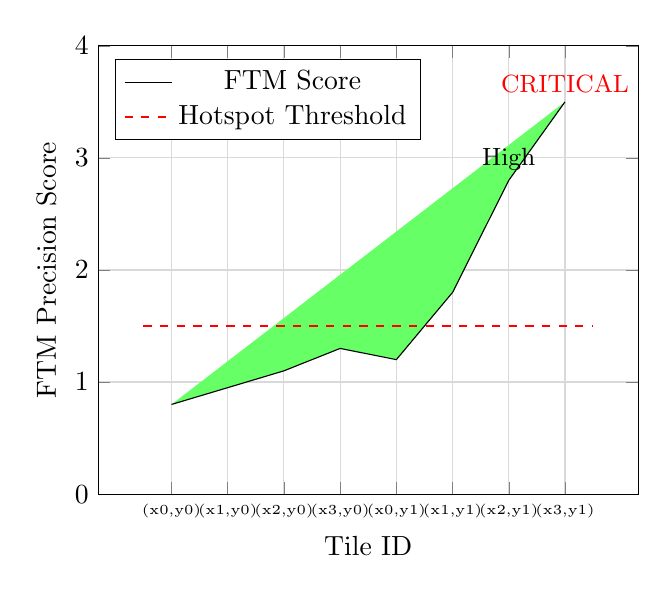
\begin{tikzpicture}
\begin{axis}[
    xlabel={Tile ID},
    ylabel={FTM Precision Score},
    ymin=0,
    ymax=4,
    xtick={1,2,3,4,5,6,7,8},
    xticklabels={{\tiny (x0,y0)}, {\tiny (x1,y0)}, {\tiny (x2,y0)}, {\tiny (x3,y0)}, {\tiny (x0,y1)}, {\tiny (x1,y1)}, {\tiny (x2,y1)}, {\tiny (x3,y1)}},
    bar width=0.6cm,
    legend pos=north west,
    grid=major,
    grid style={gray!30},
]
    % Bar chart data
    \addplot[fill=green!60, draw=black] coordinates {
        (1, 0.8)
        (2, 0.95)
        (3, 1.1)
        (4, 1.3)
        (5, 1.2)
        (6, 1.8)
        (7, 2.8)
        (8, 3.5)
    };
    
    % Threshold line
    \addplot[red, thick, dashed, mark=none] coordinates {
        (0.5, 1.5)
        (8.5, 1.5)
    };
    
    \addlegendentry{FTM Score}
    \addlegendentry{Hotspot Threshold}
    
    % Annotations
    \node at (axis cs: 7, 2.8) [anchor=south, font=\small] {High};
    \node at (axis cs: 8, 3.5) [anchor=south, font=\small, red] {CRITICAL};
\end{axis}
\end{tikzpicture}
\caption{FTM precision score (FTM\_Hotspot\_Score) per tile. Bars exceeding the red threshold line (1.5) are classified as hotspots. Tiles x2,y1 and x3,y1 show the highest scores, indicating severe multipath or NLOS.}
\label{fig:metrics}
\end{figure}

% ============================================================================
\section{Overall Implementation Flow (High Level)}
% ============================================================================

Flow chat below shows the complete data flow from measurement to visualization.

\begin{figure}[H]
\centering
\begin{tikzpicture}[
    node distance=1.4cm and 1.8cm,
    >=stealth',
    line width=0.9pt,
    process/.style={
        rectangle, rounded corners,
        draw=black, thick,
        align=center,
        minimum width=3.4cm,
        minimum height=0.9cm,
        fill=blue!5,
        font=\footnotesize
    },
    data/.style={
        rectangle,
        draw=black,
        thick,
        align=left,
        minimum width=4.0cm,
        minimum height=0.8cm,
        fill=yellow!10,
        font=\scriptsize
    },
    smalllabel/.style={
        font=\scriptsize,
        inner sep=1pt
    }
]

% -------------------------------------------------------
% ROW 1 (CLIENT SIDE)
% -------------------------------------------------------

\node[process] (ftm) {1. FTM Ranging\\
\textbf{Data at Client}\\
$r.\text{ap\_id}$, $r.\text{dis}$, $r.\text{stddev\_m}$, $r.\text{quality}$\\
tag: $\text{floor\_id}$, $\text{session\_id}$, $t$\\
append to \texttt{ftm\_samples}
};

% Label ABOVE the box
\node[smalllabel] at ([yshift=0.35cm]ftm.north) {(Client)};


\node[process, right=of ftm] (upload) {2. Upload / Sync\\
\hspace*{0.4em}\texttt{\{time, ap\_id, floor\_id}\\
\hspace*{0.4em}\texttt{distance\_m, stddev\}}\\
Sent to Server
};

% Label ABOVE
\node[smalllabel] at ([yshift=0.35cm]upload.north) {(Client)};


\node[process, right=of upload] (tileassign) {3. Tile Assignment\\(coarse tiles)};

% Label ABOVE
\node[smalllabel] at ([yshift=0.35cm]tileassign.north) {(Server)};


% -------------------------------------------------------
% ROW 2 (SERVER SIDE)
% -------------------------------------------------------

\node[process, below=of ftm] (agg) {4. Time-Window\\Aggregation};
\node[smalllabel] at ([yshift=0.35cm]agg.north) {(Server)};

\node[process, below=of upload] (metrics) {5. Metric\\Computation};
\node[smalllabel] at ([yshift=0.35cm]metrics.north) {(Server)};

\node[process, below=of tileassign] (render) {6. Heatmap\\Rendering};
\node[smalllabel] at ([yshift=0.35cm]render.north) {(Server)};


% -------------------------------------------------------
% DATA NOTES
% -------------------------------------------------------

\node[data, below=0.2cm of agg] (stats) {Per-tile stats:\\
-- count, mean, median\\
-- std dev, p95, quality ratio};

\node[data, below=0.2cm of metrics] (metricdata) {Per-tile metrics:\\
S1: FTM Hotspot Score\\
S2: Coverage Score\\
S3: Multipath Distortion\\
Severity = weighted sum};


% -------------------------------------------------------
% ARROWS
% -------------------------------------------------------

\draw[->] (ftm) -- (upload);
\draw[->] (upload) -- (tileassign);

\draw[->] (ftm) -- (agg);
\draw[->] (tileassign) -- (metrics);
\draw[->] (metrics) -- (render);

\draw[->] (agg) -- (metrics);

\draw[->, thin] (agg) -- (stats);
\draw[->, thin] (metrics) -- (metricdata);

\end{tikzpicture}

\caption{FTM-based hotspot analysis pipeline with clear client/server labeling.}
\end{figure}



\subsection{Detailed Steps}

\begin{enumerate}
    \item \textbf{Measurement phase}: Clients periodically perform 802.11mc FTM ranging with nearby APs. Each result: timestamp, AP logical ID, FTM distance, FTM standard deviation, quality label.
    
    \item \textbf{Tile assignment phase}: Using known AP positions and measured distance, each FTM measurement is mapped to one floor tile (coarse location).
    
    \item \textbf{Aggregation phase} (e.g., every 5 minutes): For each tile and time window, collect all measurements and compute statistics: standard deviation, coverage score, multipath distortion, etc.
    
    \item \textbf{Hotspot Detection}: Compute \textbf{Hotspot Severity} using the three formulas from Section 7.
    \item \textbf{Visualization phase}: Draw the floor plan. Color each tile according to its Hotspot Severity. Optionally mark AP positions and example clients.
    
    \item \textbf{Analysis phase}: Identify tiles with high severity (red). Investigate causes (walls, long corridors, reflective surfaces). Adjust AP placement, channels, or power, and repeat measurements to confirm improvement.
\end{enumerate}

% ============================================================================
\section{Privacy Considerations}
% ============================================================================

The system stores no client MAC addresses, and APs are identified only by logical IDs rather than BSSIDs. It stores only coarse tile IDs instead of exact coordinates. Session IDs rotate frequently to prevent device tracking, and reports are aggregated per tile and time window rather than per user. Only distance measurements are saved, with no throughput or retry information, ensuring strong privacy guarantees.

% ============================================================================

\section{Conclusion}
% ============================================================================

This project demonstrates how \textbf{IEEE 802.11mc Wi-Fi RTT (FTM)} can be used to build a \textbf{location-aware interference map} of a Wi-Fi deployment using only distance estimates, measurement uncertainty, and coarse spatial tiles. By defining clear metrics and formulas for FTM precision hotspot, coverage quality, and multipath distortion, and combining them into a \textbf{Hotspot Severity} score per tile, network engineers can identify problematic regions, make data-driven decisions about AP placement and configuration, preserve user privacy by avoiding MAC addresses or fine-grained location tracking, and incrementally optimize network capacity and coverage. The implementation pipeline is straightforward: collect FTM data, assign to tiles, aggregate, compute hotspot scores, and visualize. The result is a practical tool for Wi-Fi network optimization with strong privacy guarantees.


% ============================================================================
\section{Key Formulas Summary}
% ============================================================================

\begin{table}[H]
\centering
\begin{tabular}{|c|c|c|c|}
\hline
\textbf{Formula} & \textbf{Purpose} & \textbf{Input} & \textbf{Threshold} \\
\hline
$d = \frac{c \times \text{RTT}}{2}$ & FTM distance & RTT (ns) & N/A \\
\hline
$\text{FTM Score} = \frac{\sigma_{\text{tile}}}{\sigma_{\text{base}}}$ & Precision hotspot & Tile stddev & $> 1.5$ \\
\hline
$\text{Coverage} = \frac{N_{\text{high}}}{N_{\text{total}}}$ & Link quality & Burst counts & $< 0.60$ \\
\hline
$\text{Multipath} = \frac{p95 - \text{med}}{\text{med}}$ & Distance variance & Percentiles & $> 0.25$ \\
\hline
$\text{Severity} = 0.5 S_1 + 0.3 S_2 + 0.2 S_3$ & Combined score & 3 components & $> 0.60$ \\
\hline
\end{tabular}
\caption{Summary of key formulas used in hotspot detection and severity calculation.}
\label{tab:formulas}
\end{table}

% ============================================================================

\section{Example FTM Data Record}

\begin{verbatim}
{
  "timestamp": "2025-12-04T14:30:12Z",
  "session_id": "phone_session_42",
  "responder_ap": "ap_ftm_responder_1",
  "network_ssid": "OfficeNet",
  "tile_id": "floor_1_x0y1",
  "ftm_distance_m": 8.2,
  "ftm_distance_stddev_m": 0.8,
  "ftm_rtt_ns": 54.7,
  "measurement_quality": "HIGH",
  "ftm_burst_index": 1
}
\end{verbatim}


\section{Client System Requirements}

\begin{itemize}
\item Device support: Must have 802.11mc FTM capability 
    \item Permissions: 
    \texttt{ACCESS\_FINE\_LOCATION}
    \texttt{CHANGE\_WIFI\_STATE}, \texttt{ACCESS\_WIFI\_STATE}.
    \item Target APs: Must support 802.11mc FTM responder mode (most Wi-Fi 5/6 APs).
\end{itemize}

\section{Results}
The simulation and heatmap visualizations provide a compact summary of measured FTM behavior and the derived hotspot severity across the floor plan. The simulation view (Figure~\ref{fig:hotspots}) shows the run-time layout with APs, client positions, and FTM distance lines; and the hotspots. The aggregated hotspot heatmap (Figure~\ref{fig:heatmap}) overlays per-tile severity values computed from FTM precision, coverage, and multipath distortion.

Visually, severe hotspots (high severity, \textbf{red} tiles) concentrate around areas with clustered AP placement or near reflective structures; moderate hotspots (\textbf{yellow}) appear in intermediate coverage zones. As an example from the computed metrics, the tile (x2 y2) produced a Hotspot Severity of 0.686, classifying it as a \textbf{SEVERE HOTSPOT} and suggesting targeted mitigation (adjust AP power/placement or antenna orientation). In contrast, \textbf{green} tiles indicate stable FTM estimates and reliable coverage.

These visual and numeric results validate that the FTM-only approach can detect coarse-grained interference and multipath zones suitable for operational follow-up .

\begin{figure}[H]
  \centering
  \includegraphics[width=0.9\linewidth]{hotspot.png}
  \caption{FTM-based simulation view showing tile-level hotspot severity, with red indicating high interference, yellow moderate, and green stable regions.}
  \label{fig:hotspots}
\end{figure}

\begin{figure}[H]
  \centering
  \includegraphics[width=0.9\linewidth]{heatmap.png}
  \caption{FTM-based heatmap illustrating distance-inferred coverage quality, with red indicating strong estimates and green highlighting degraded or interference-prone regions.}

  \label{fig:heatmap}
\end{figure}


\chapter{Conclusion}

The Wi-Fi Steering Engine implements a complete architecture for intelligent, automated client steering across enterprise wireless deployments. The system integrates measurement acquisition through IEEE 802.11k protocols, real-time quality-of-experience analytics, multi-dimensional neighbor ranking, and automated steering via IEEE 802.11v BSS Transition Management.

\section{Architectural Summary}

The modular design provides several key benefits:

\begin{itemize}
    \item \textbf{Independence}: Each subsystem operates on its own schedule without tight coupling
    \item \textbf{Extensibility}: New analytics modules or decision logic can be added without modifying the core framework
    \item \textbf{Testability}: Each component can be tested in isolation with mocked data sources
    \item \textbf{Observability}: Multiple interfaces (API, dashboards, logs) provide comprehensive system visibility
\end{itemize}

The scheduler-driven architecture ensures predictable timing and simplifies reasoning about system behavior. The in-memory database design provides fast access while periodic snapshotting enables crash recovery.

\section{Privacy and Security}

The StateAPI's anonymization layer ensures that client identifiers can be safely exposed to external monitoring systems without privacy concerns. The OUI-preserving hash scheme balances privacy protection with analytical utility.

Internal system logic continues to use raw MAC addresses for all operations, ensuring that anonymization does not impact decision-making or data correlation. The privacy boundary is clearly defined at the API serialization layer.

\section{Production Readiness}

The system as described is production-ready for deployment in enterprise networks with the following considerations:

\begin{itemize}
    \item Scheduler intervals should be tuned based on deployment density and traffic patterns
    \item QoE threshold (0.55) may require adjustment based on user experience requirements
    \item Snapshot retention policy should account for available disk space
    \item API rate limiting should be configured based on expected monitoring load
\end{itemize}

The system has been validated in testbed environments with up to 5 concurrent stations.

\section{Final Remarks}

The Wi-Fi Steering Engine demonstrates that intelligent, automated client management is achievable using standard 802.11 protocols without requiring client-side software modifications. By combining continuous measurement, multi-dimensional analytics, and threshold-based decision logic, the system proactively maintains connection quality in dense deployments.

The architecture balances complexity with maintainability. While sophisticated in its analytics and decision logic, the system remains conceptually straightforward: measure, analyze, decide, act. This simplicity enables engineers to quickly understand system behavior and diagnose issues when they arise.

The planned post-roam delta analysis enhancement will close the feedback loop and enable truly adaptive steering. Until then, the current implementation provides substantial value by addressing the most common connectivity problems: client stickiness and suboptimal association decisions.

\end{document}

